\section{Numerical Evidence for Resolvent-Mediated Newtonian Response}

  \subsection{Discrete Model}

    We approximate a three-dimensional Laplace-type operator by the
    graph Laplacian $L$ on a cubic lattice with Dirichlet boundary conditions.
    The operator used in the simulations is
    \begin{equation}
      A = L + \varepsilon I,
    \end{equation}
    with $\varepsilon > 0$ small enough to remove the zero mode while
    preserving the long-distance behavior of the Green kernel.

    A localized perturbation is introduced by symmetrically modifying
    edge weights inside a ball of lattice radius $R$.
    The perturbed operator reads
    \begin{equation}
      A \longrightarrow A + \delta A,
    \end{equation}
    with $\delta A$ compactly supported.

    The Green column associated with a point source is computed by solving
    \begin{equation}
      A \phi = \delta_{\mathrm{source}},
    \end{equation}
    and the radial profile of $\phi$ is fitted at large distance by
    \begin{equation}
      \phi(r) \sim \frac{a}{r} + b.
    \end{equation}
    The coefficient $a$ characterizes the effective Newtonian amplitude.

  \subsection{Verification of the First-Order Entropy Variation}

    For weak perturbations, the identity
    \begin{equation}
      \Delta \log \det{}' A
      \approx
      \mathrm{Tr}((A^{-1})_{SS} \delta A_{SS})
    \end{equation}
    was evaluated numerically on the support $S$ of the perturbation.

    Across the tested parameter range,
    the ratio between the exact support-restricted log-determinant variation
    and the resolvent trace remained close to unity
    (typically within a few percent for small perturbations).
    This confirms that the weak-field expansion
    \begin{equation}
      \delta S_\Pi = \tfrac12 \mathrm{Tr}(A^{-1}\delta A)
    \end{equation}
    is accurately realized in the discrete setting.

  \subsection{Spatial Support Threshold}

    The central result concerns the dependence of the Newtonian amplitude
    shift $\Delta a$ on the spatial support of the perturbation.

    For perturbations confined to a small region ($R=1$),
    the entropy variation $\Delta \log \det{}' A$ is clearly non-zero,
    yet the fitted amplitude $a$ remains essentially unchanged.
    The modification of the spectrum is therefore spectrally local
    and does not generate a measurable long-range effect.

    For intermediate support ($R=2$),
    the amplitude shift remains very small over the tested range.

    In contrast, for perturbations extending over a larger region
    ($R=3$ in the simulations),
    a coherent and monotonic modification of the Newtonian amplitude emerges.
    The amplitude shift $\Delta a$ increases in magnitude
    as $-\Delta \log \det{}' A$ grows,
    as shown in Fig.~\ref{fig:deltaa_logdet}.

    \begin{figure}
      \centering
      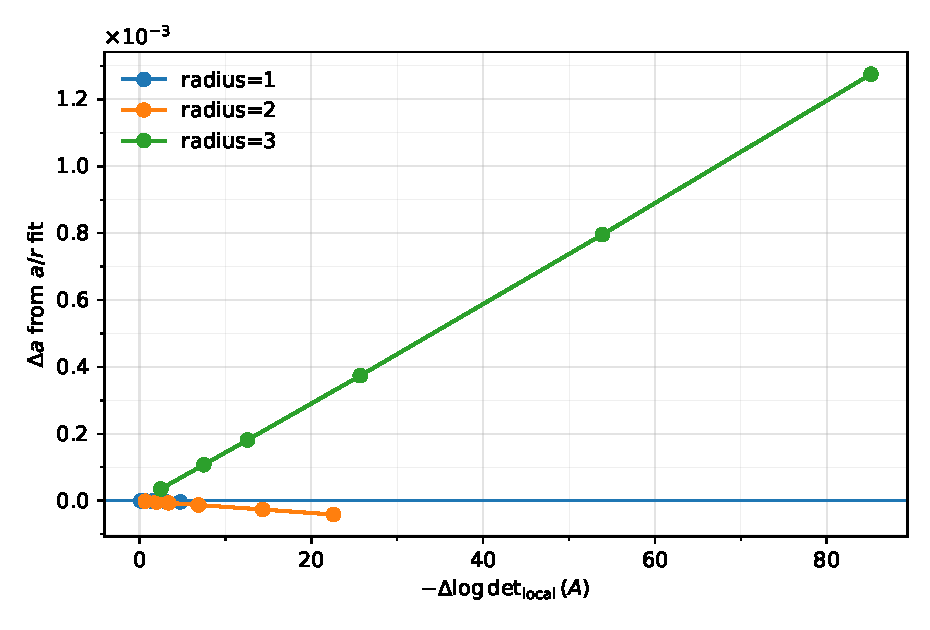
\includegraphics[width=0.8\linewidth]{04-spatial-support/fig_deltaa_vs_neg_dlogdet_by_radius}
      \caption{
        Shift of the fitted Newtonian amplitude $\Delta a$
        as a function of $-\Delta \log \det{}' A$
        for perturbations of increasing spatial radius $R$.
        Only sufficiently extended perturbations produce
        a macroscopic long-range response.
      }
      \label{fig:deltaa_logdet}
    \end{figure}

    These results demonstrate that entropy variation alone is not sufficient
    to produce a Newtonian interaction.
    A finite spatial coherence of the perturbation is required
    for the resolvent-mediated response to propagate to large distances.
